\documentclass{article}
\usepackage[T1]{fontenc}
\usepackage{lmodern}
\usepackage{graphicx}
\usepackage{amsmath,amssymb}
\usepackage[a4paper,margin=2cm]{geometry}
\usepackage[absolute,overlay]{textpos}
\setlength{\TPHorizModule}{1mm}
\setlength{\TPVertModule}{1mm}
\usepackage[indonesian]{babel}
\usepackage{hyperref}
\setlength{\emergencystretch}{2em}
% unit: Halaman 2

\begin{document}

% === Halaman 2 (python/native) ===

2

Pendahuluan

• Algoritma Elgamal dibuat oleh Taher Elgamal (1985). Pertama kali 

dikemukakannya di dalam makalah berjudul "A public key cryptosystem and 

a signature scheme based on discrete logarithms”, dimuat di dalam IEEE 

Transactions on Information Theory ( Volume: 31, Issue: 4, July 1985)

% deskripsi: gambar native xref 35
\noindent
\includegraphics[width=0.85\textwidth]{../../images/python/page_002_img_01.jpeg}

% deskripsi: gambar native xref 36
\noindent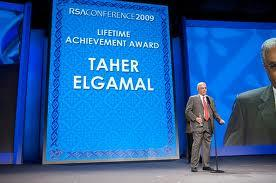
\includegraphics[width=0.85\textwidth]{../../images/python/page_002_img_02.jpeg}

\end{document}
